%%%%%%%%%%%%%%%%%%%%%%%%%%%%%%%%%%%%%%%%%%%%%%%%%%%%%%%%%%%%%%%%%%%%%%%%%%%%%%%%%%
%%                               APENDICE                                      %%
%%%%%%%%%%%%%%%%%%%%%%%%%%%%%%%%%%%%%%%%%%%%%%%%%%%%%%%%%%%%%%%%%%%%%%%%%%%%%%%%%%

\chapter{Apêndice}\label{chap:appendix}
%%%%%%%%%%%%%%%%%%%%%%%%%%%%%%%%%%%%%%%%%%%%%%%%%%%%%%%%%%%%%%%%%%%%%%%%%%%%%%%%%%
\section{Bacias de convergência}\label{section:convBasins}
  \begin{figure}[htp]
    \centering
    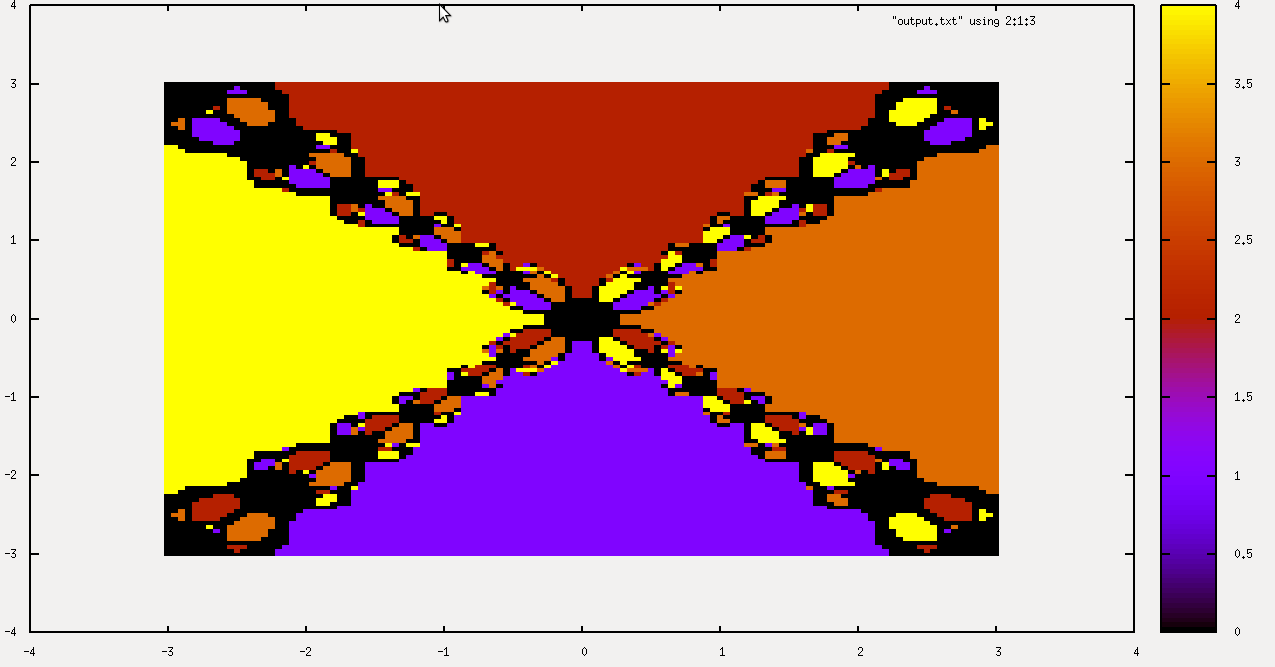
\includegraphics[width=0.9\textwidth]{imgs/img1.png}
    \caption{$f(x) = x^4 -1$ com $intervalo = [-3: 0.05: 3]$, total de 14641 pontos}
  \end{figure}

  \begin{figure}[htp]
    \centering
    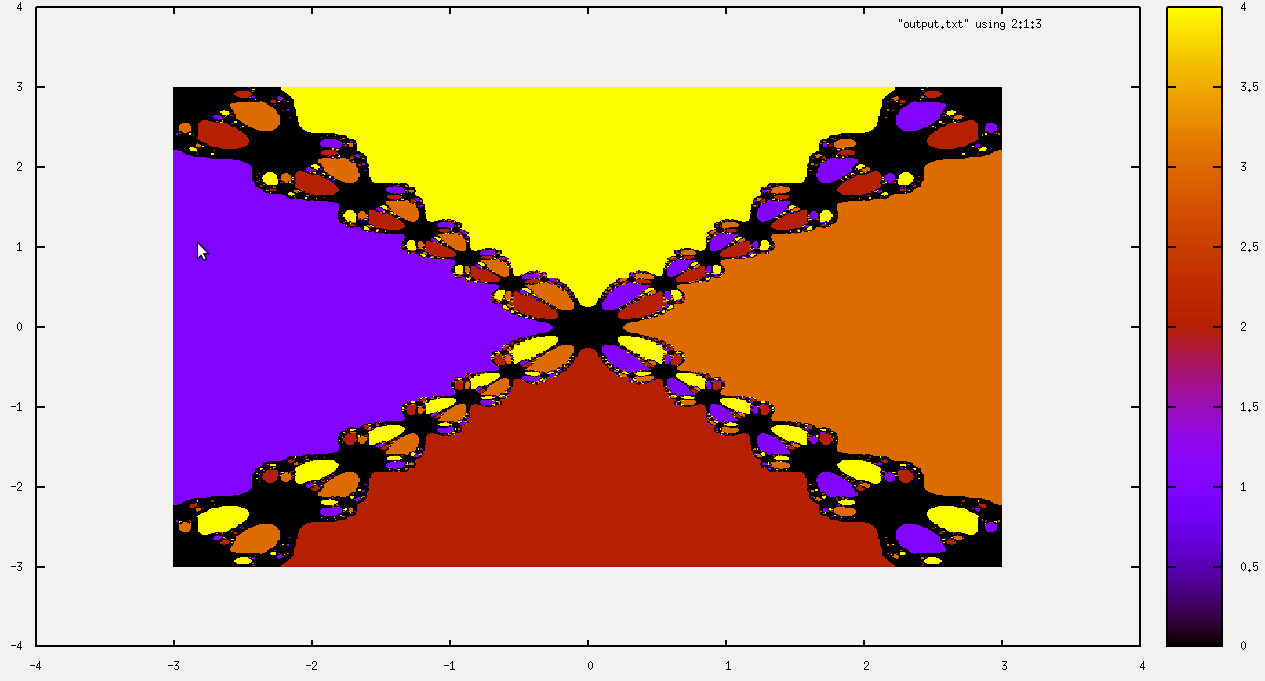
\includegraphics[width=0.9\textwidth]{imgs/img2.png}
    \caption{$f(x) = x^4 -1$ com $intervalo = [-3: 0.01: 3]$, total de 361201 pontos}
  \end{figure}

  \begin{figure}[htp]
    \centering
    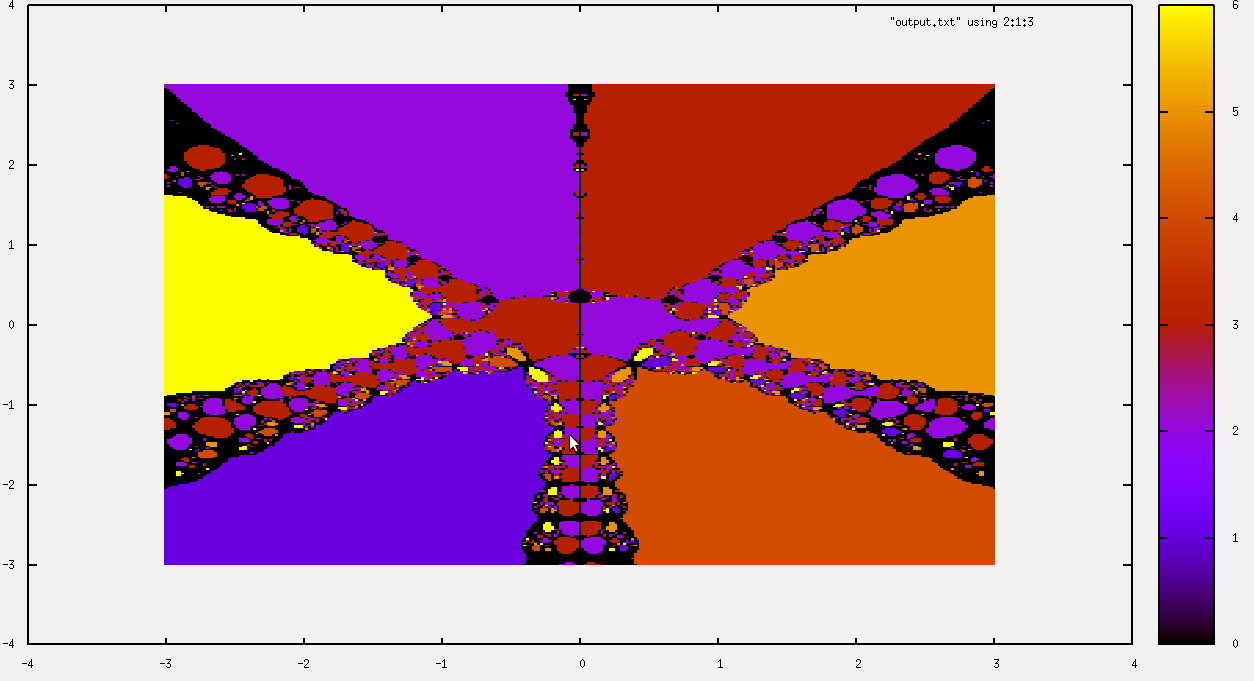
\includegraphics[width=0.9\textwidth]{imgs/img3.png}
    \caption{$f(x) = x^6 + 1*x^4 - 1*x^2 - 2*x^1 + 2$ com $intervalo = [-3: 0.02: 3]$, total de 90601 pontos}
  \end{figure}

  \begin{figure}[htp]
    \centering
    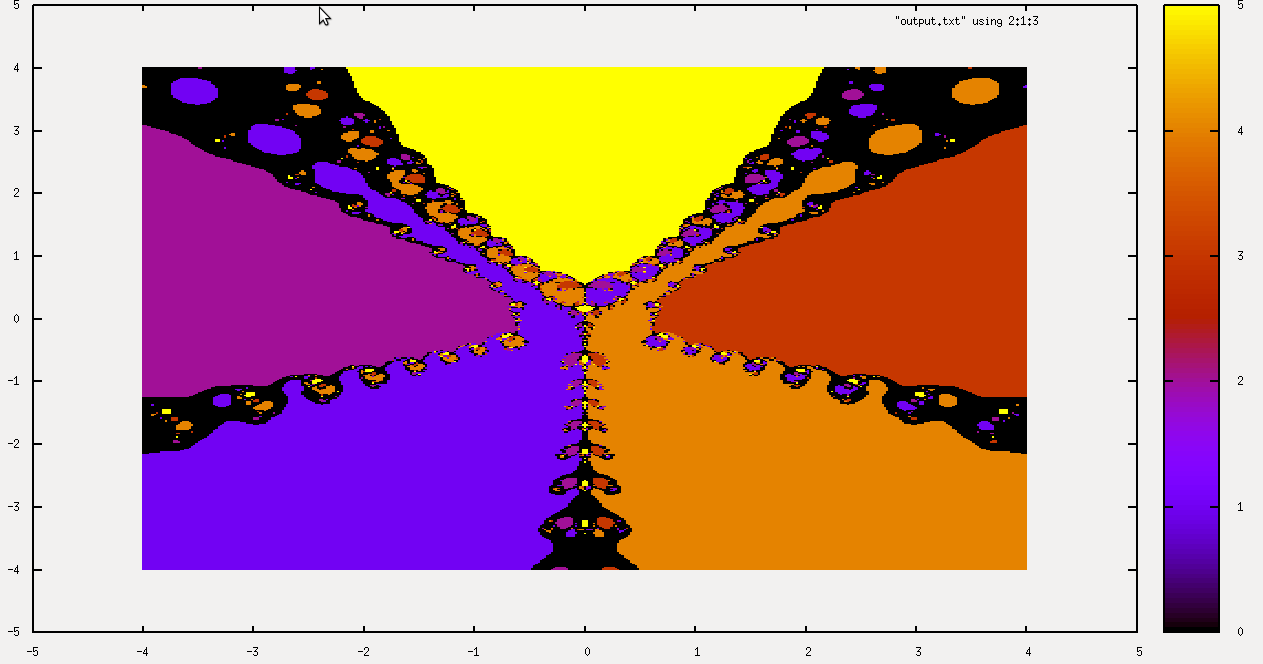
\includegraphics[width=0.9\textwidth]{imgs/img4.png}
    \caption{$f(x) = 3*x^5 + 2*x^4 + 1*x^3 - 1*x^2 - 2*x^1 - 3$ com $intervalo = [-4: 0.02: 4]$, total de 160801 pontos}
  \end{figure}

  \begin{figure}[htp]
    \centering
    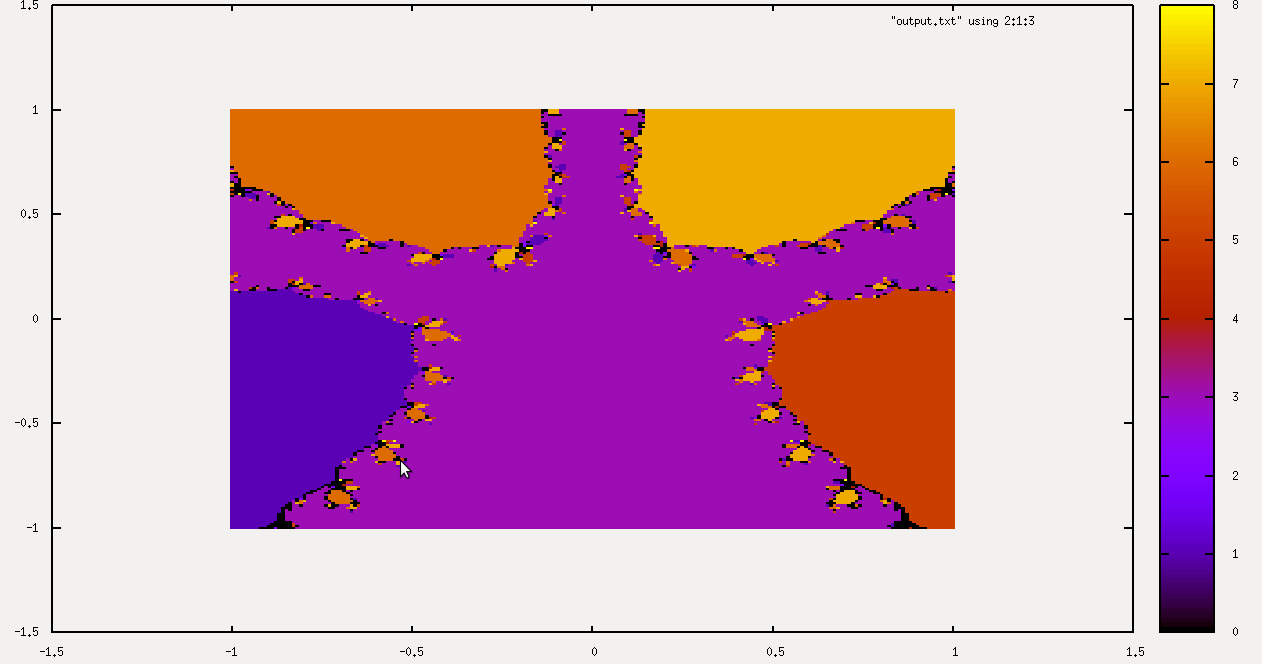
\includegraphics[width=0.9\textwidth]{imgs/img5.png}
    \caption{$f(x) = 1*x^8 + 1*x^6 + 5*x^5 - 4*x^4 + 3*x^3 - 2*x^2 + 1*x^1$ com $intervalo = [-1: 0.01: 1]$, total de 40401 pontos}
  \end{figure}

  \begin{figure}[htp]
    \centering
    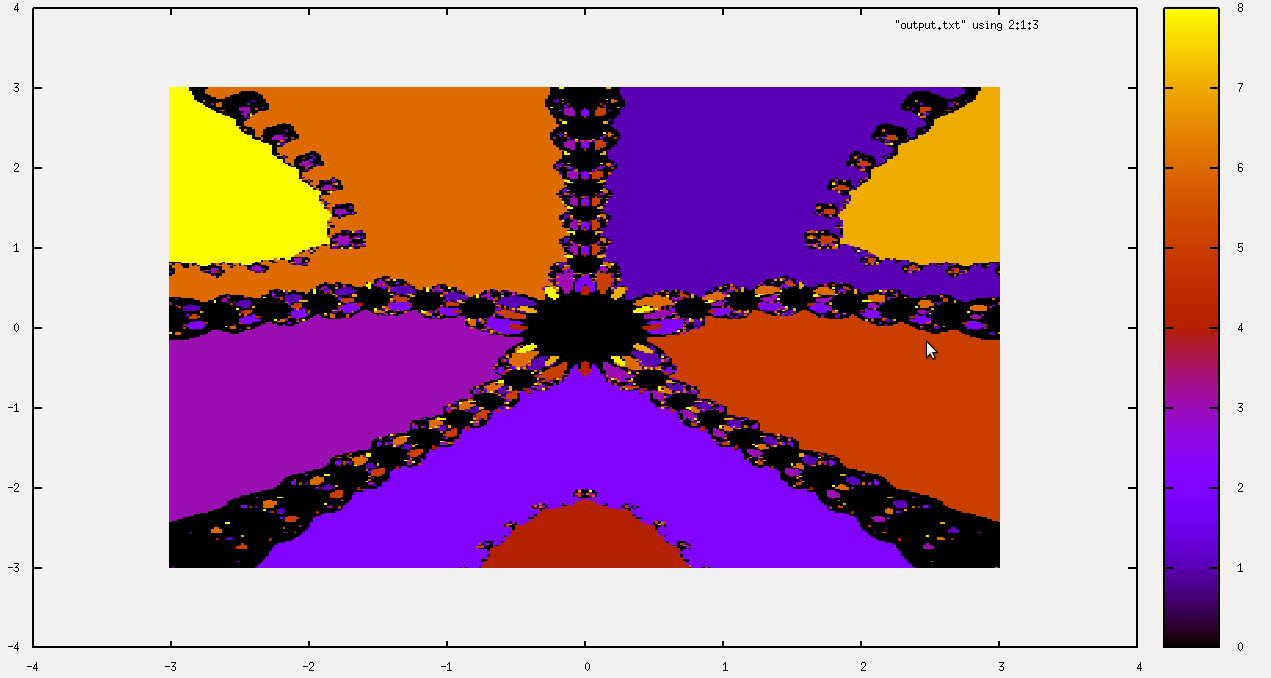
\includegraphics[width=0.9\textwidth]{imgs/img6.png}
    \caption{$f(x) = 1*x^8 + 15*x^5 + 16$ com $intervalo = [-3: 0.02: 3]$, total de 90601  pontos}
  \end{figure}

  \section{Todas as raízes de uma função}\label{section:allRoots}
    
    \begin{verbatim}
      $ octave n_roots_function.m
      Choise: 1
      Interval: [a:step:b] -- [ -10 : 0.050000 : 10 ]
      Points: 401
      Interval #7: ]2, 4] has root 2.35755105
      Interval #10: ]8, 10] has root 8.50719957

      $ octave n_roots_function.m
      Choise: 2
      Interval: [a:step:b] -- [ -10 : 0.050000 : 10 ]
      Points: 401
      Interval #1: ]-10, -8] has root -9.42477796
      Interval #2: ]-8, -6] has root -6.28318530
      Interval #4: ]-4, -2] has root -3.14159265
      Interval #7: ]2, 4] has root 3.14159265
      Interval #9: ]6, 8] has root 6.28318531
      Interval #10: ]8, 10] has root 9.42477796

      $ octave n_roots_function.m
      Choise: 3
      Interval: [a:step:b] -- [ -10 : 0.050000 : 10 ]
      Points: 401
      Interval #4: ]-4, -2] has root -3.00000000
      Interval #6: ]0, 2] has root 1.00000000
      f(x) = 1*x^2 + 2*x^1 - 3

      $ octave n_roots_function.m
      Choise: 3
      Interval: [a:step:b] -- [ -10 : 0.050000 : 10 ]
      Points: 401
      Interval #4: ]-4, -2] has root -2.30277564
      Interval #5: ]-2, 0] has root -1.61803399
      Interval #6: ]0, 2] has root 0.61803399
      Interval #6: ]0, 2] has root 1.30277564
      f(x) = 1*x^4 + 2*x^3 - 3*x^2 - 4*x^1 + 3

      $ octave n_roots_function.m
      Choise: 3
      Interval: [a:step:b] -- [ -10 : 0.050000 : 10 ]
      Points: 401
      Interval #6: ]0, 2] has root 0.67078673
      Interval #6: ]0, 2] has root 0.84877121
      f(x) = 1*x^6 + 1*x^5 + 1*x^4 + 2*x^3 - 3*x^2 - 4*x^1 + 3
    \end{verbatim}
